% Chapter Template

\chapter{Numerical Analysis} % Main chapter title

\label{Chapter3} % Change X to a consecutive number; for referencing this chapter elsewhere, use \ref{ChapterX}

\lhead{Chapter 3. \emph{Numerical Analysis}} % Change X to a consecutive number; this is for the header on each page - perhaps a shortened title

\section{Linear Stability Analysis}
Let's consider the following for analyzing the methods:
    \begin{itemize}
        \item Resistor R=10 $\Omega$
        \item Inductor L=1mH
        \item For the input square wave $v_{in}$:\\
        Amplitude $v_{0}=5V$\\
        Time Period T=1ms\\
        Duty Ratio $\alpha$ =0.5
    \end{itemize}
    The square wave input:\\
    \[
        V(t) =
        \begin{cases}
        5 \, \text{V}, & \text{if } 0 \leq t < 0.5 \, \text{ms} \\
        0 \, \text{V}, & \text{if } 0.5 \, \text{ms} \leq t < 1 \, \text{ms}
        \end{cases}
    \]
    and the governing equation after substituting R and L values is \[\frac{di(t)}{dt}=1000v_{in}(t)-10000i(t)\]\\
    For the RL equation the eigenvalue $\lambda=-\frac{R}{L}=-10000$.\\
\begin{enumerate}
    \item \textbf{RK-2}\\
    The stability function for RK-2 is:
    \begin{equation}
        R(z)=1+z+ \frac{z^2}{2}
    \end{equation}
    where $z=h \lambda$ and the condition for stability is $|R(z)| \leq 1$.\\
    On solving the equation $\lambda =-\frac{R}{L}$.
    Substituting the value of $\lambda$ into stability condition:
    \begin{equation}
        |1-h \frac{R}{L}+\frac{(h \frac{R}{L})^2}{2}| \leq 1
    \end{equation}
    
    Now, substituting $\lambda=-10000$ into the stability condition:
    \begin{equation}
        |1+h(-10000)+\frac{(h(-10000))^2}{2}| \leq 1
    \end{equation}
    \textbf{Conclusion:} RK-2 is conditionally stable for \( h \leq 0.0002 \, \text{s} \)

    
    \item \textbf{Forward Euler}\\
    The Forward Euler method approximates the solution as:
    \begin{equation}
        i_{n+1} = i_n + h \lambda i_n = (1 + h \lambda) i_n.
    \end{equation}
    The stability condition is:
    \begin{equation}
        |1 + h \lambda| \leq 1.
    \end{equation}
    Substituting \( \lambda = -10000 \) from the example before:
    \begin{equation}
        |1 - 10000 h| \leq 1 \implies h \leq 0.0002 \, \text{s}.
    \end{equation}
    \textbf{Conclusion:} Forward Euler is conditionally stable for \( h \leq 0.0002 \, \text{s} \).
    

    \item \textbf{Backward Euler}\\
    The Backward Euler method approximates the solution as:
    \begin{equation}
        i_{n+1} = i_n + h \lambda i_{n+1} \implies i_{n+1} = \frac{i_n}{1 - h \lambda}.
    \end{equation}
    The stability condition is:
    \begin{equation}
        \left| \frac{1}{1 - h \lambda} \right| \leq 1.
    \end{equation}
    Since \( \lambda = -10000 \), this becomes:
    \begin{equation}
        \left| \frac{1}{1 + 10000 h} \right| \leq 1,
    \end{equation}
    which is always true for \( h > 0 \).\\
    \textbf{Conclusion:} Backward Euler is unconditionally stable.


    \item \textbf{RK-4}\\
    The RK-4 method has the stability function:
    \begin{equation}
        R(z) = 1 + z + \frac{z^2}{2} + \frac{z^3}{6} + \frac{z^4}{24}, \quad z = h \lambda.
    \end{equation}
    The stability condition is:
    \begin{equation}
        |R(z)| \leq 1.
    \end{equation}
    Substituting \( \lambda = -10000 \):
    \begin{equation}
        |R(-10000 h)| \leq 1 \implies h \leq 0.0002785 \, \text{s}.
    \end{equation}
    \textbf{Conclusion:} RK-4 is conditionally stable for \( h \leq 0.0002785 \, \text{s} \).


    \item \textbf{Trapezoidal Method}\\
    The Trapezoidal method approximates the solution as:
    \begin{equation}
        i_{n+1} = i_n + \frac{h}{2} (\lambda i_n + \lambda i_{n+1}) \implies i_{n+1} = \frac{1 + \frac{h \lambda}{2}}{1 - \frac{h \lambda}{2}} i_n.
    \end{equation}
    The stability condition is:
    \begin{equation}
        \left| \frac{1 + \frac{h \lambda}{2}}{1 - \frac{h \lambda}{2}} \right| \leq 1.
    \end{equation}
    Substituting \( \lambda = -10000 \):
    \begin{equation}
        \left| \frac{1 - 5000 h}{1 + 5000 h} \right| \leq 1,
    \end{equation}
    which is always true for \( h > 0 \).\\
    \textbf{Conclusion:} The Trapezoidal method is unconditionally stable.

\end{enumerate}

\section{Showcase of Stability Regions}
\begin{figure}[H]
  \centering
  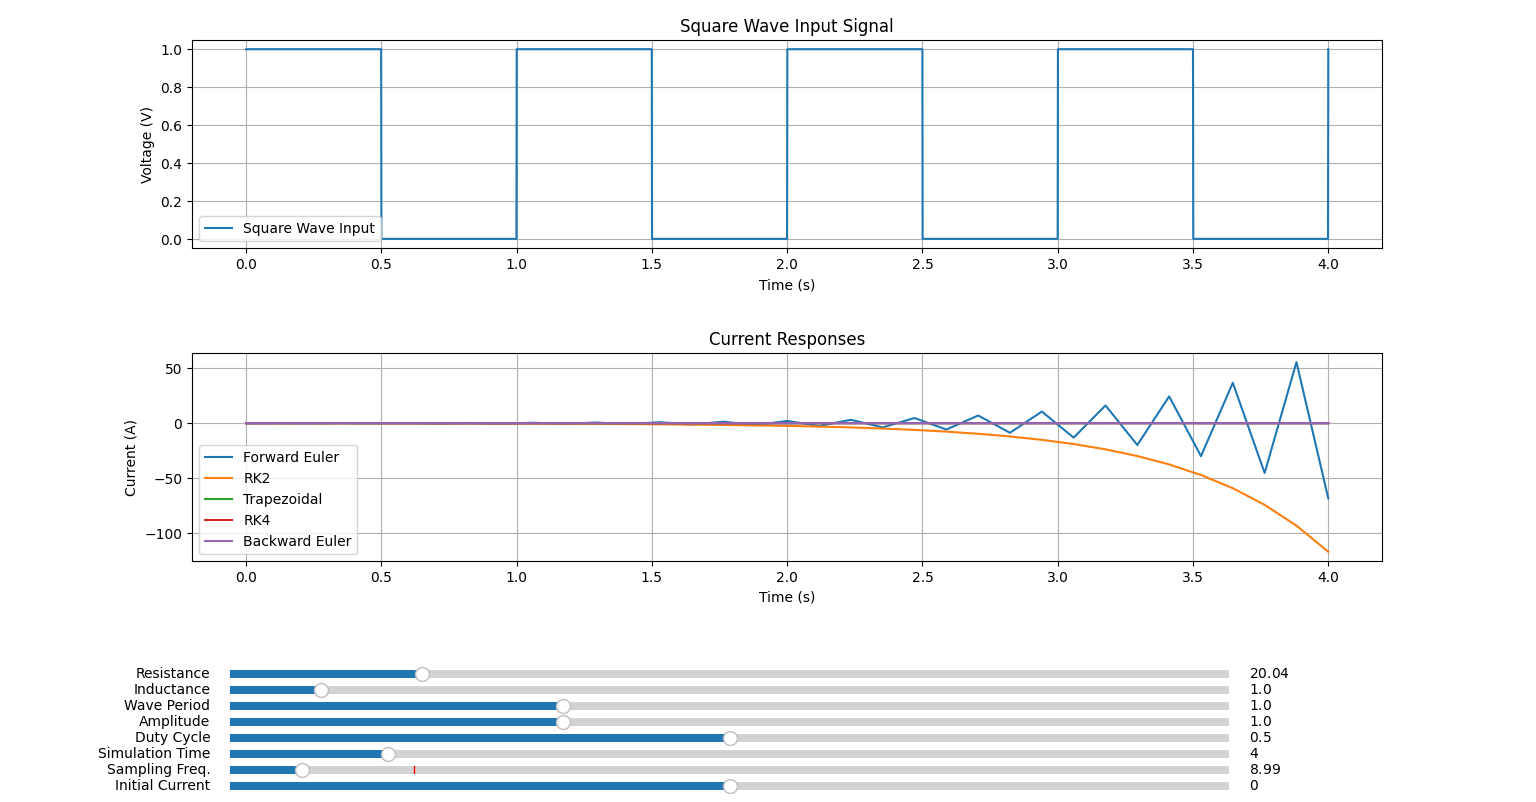
\includegraphics[width=\textwidth]{figs/instability_fwd_euler.png}
  \caption{Instability of the Forward Euler method for a step size that violates the stability condition.}
  \label{fig:instability_forward_euler}
\end{figure}

\begin{figure}[H]
  \centering
  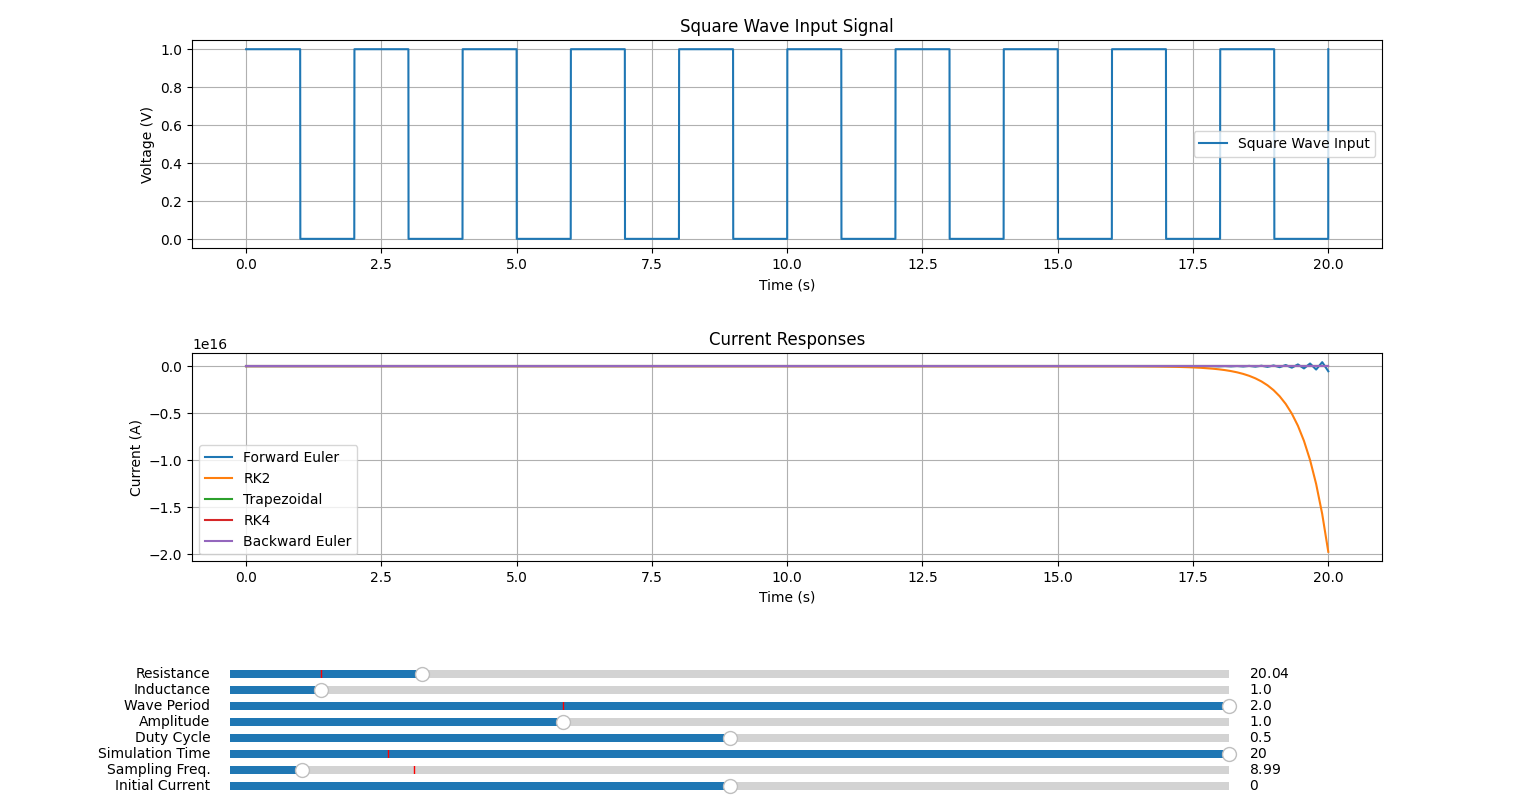
\includegraphics[width=\textwidth]{figs/instability_rk2.png}
  \caption{Instability behavior of RK2 (Heun's) method when the step size is too large.}
  \label{fig:instability_rk2}
\end{figure}


\begin{figure}[H]
  \centering
  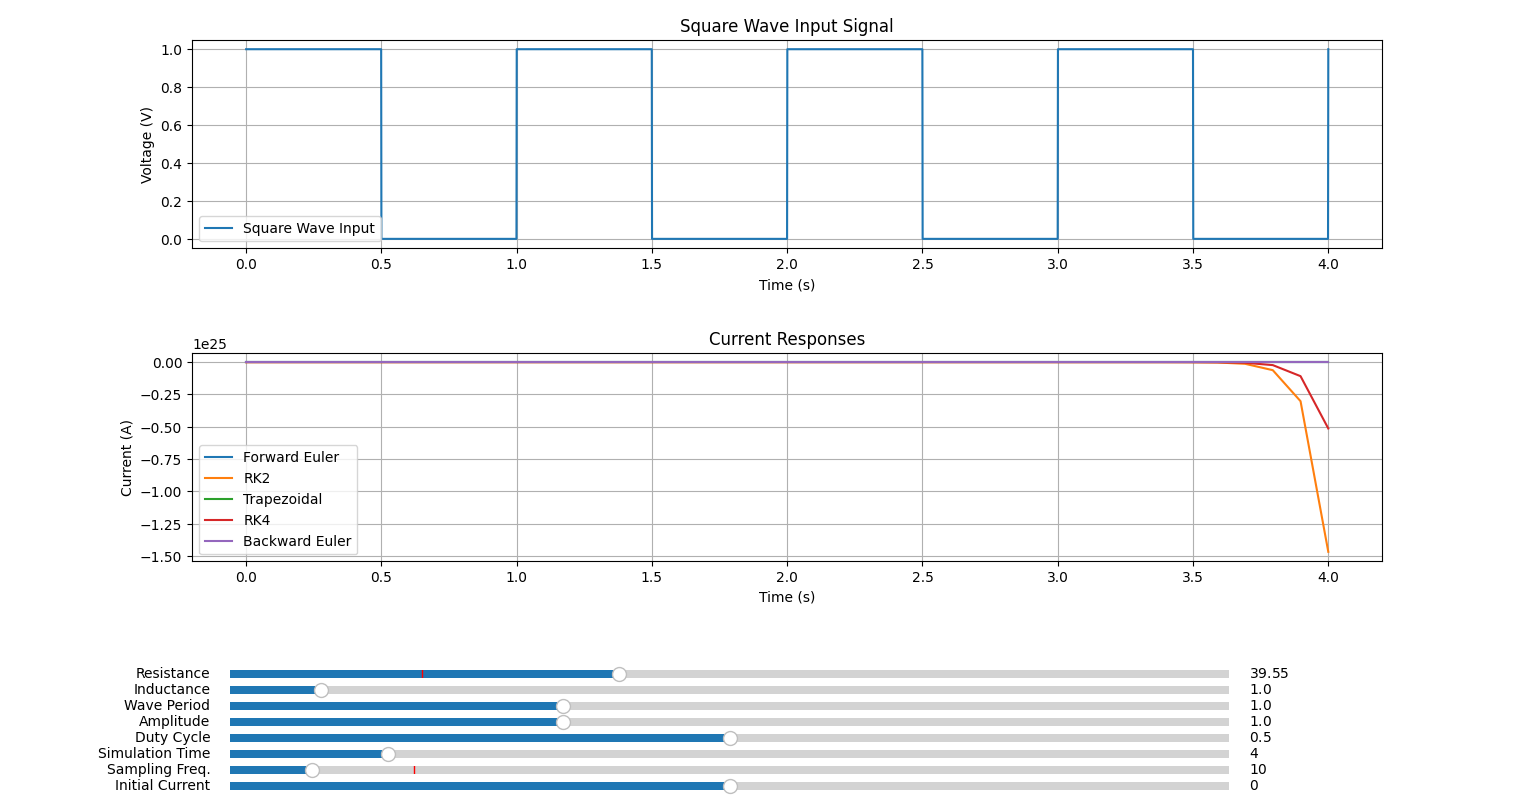
\includegraphics[width=\textwidth]{figs/instability_rk4.png}
  \caption{Instability behavior of RK4 when the step size exceeds the stability region (bounded region).}
  \label{fig:instability_rk4}
\end{figure}
\section{Local and Global Truncation Error}
\begin{figure}[H]
  \centering
  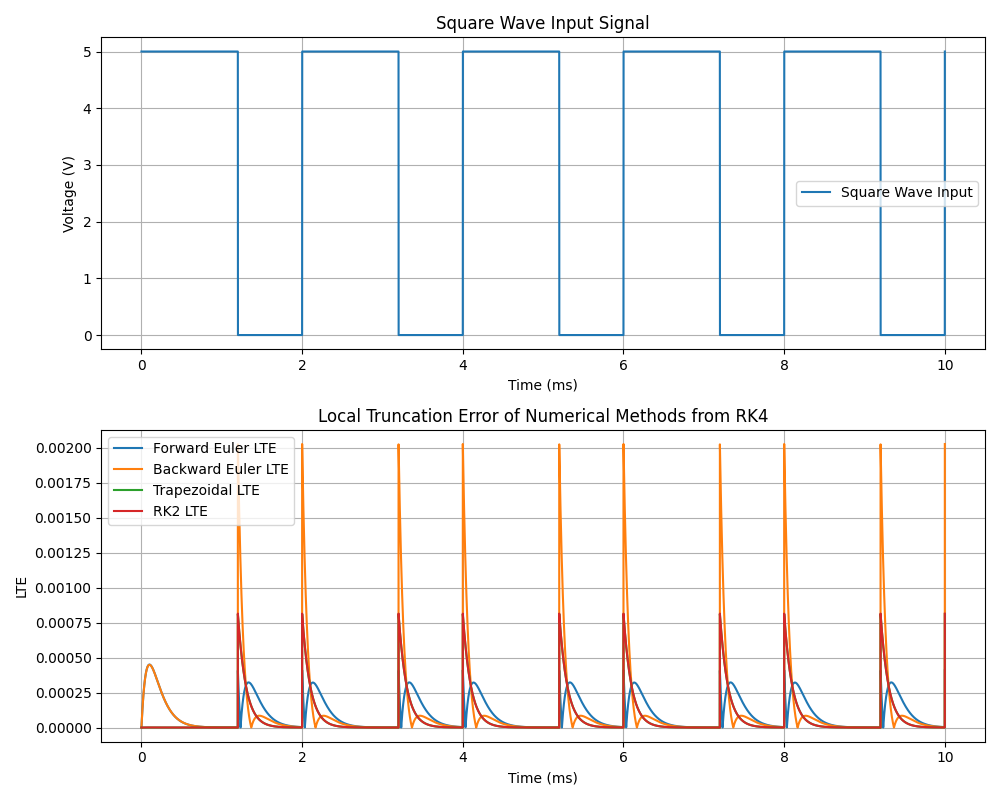
\includegraphics[width=\textwidth]{figs/local_error.png}
  \caption{Local truncation error at each sample point for selected values of $R$, $L$, and the sampling rate.}
  \label{fig:local_error}
\end{figure}

\begin{figure}[H]
  \centering
  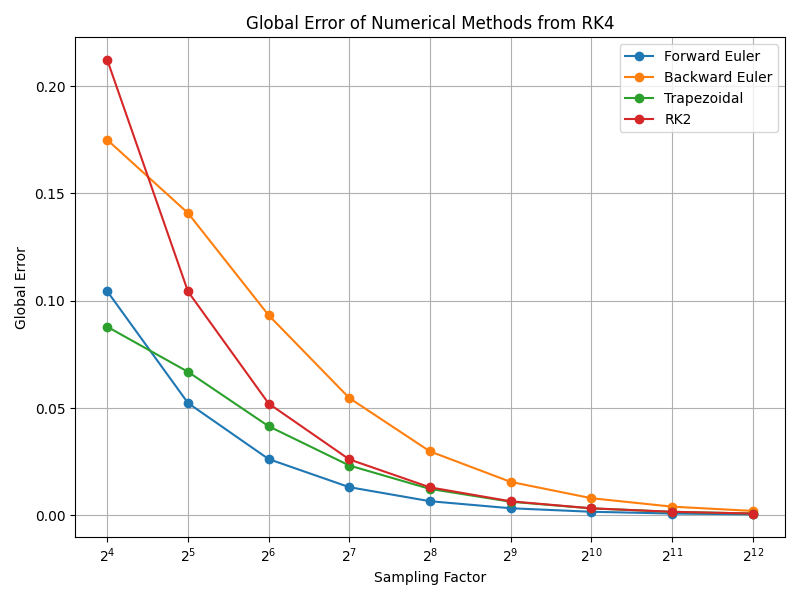
\includegraphics[width=\textwidth]{figs/global_error.png}
  \caption{Global error versus the sampling factor. The RK4 method is used as the reference due to its higher order accuracy ($O(h^4)$).}
  \label{fig:global_error}
\end{figure}
\section{Comparison of Computational Times}
\begin{figure}[H]
  \centering
  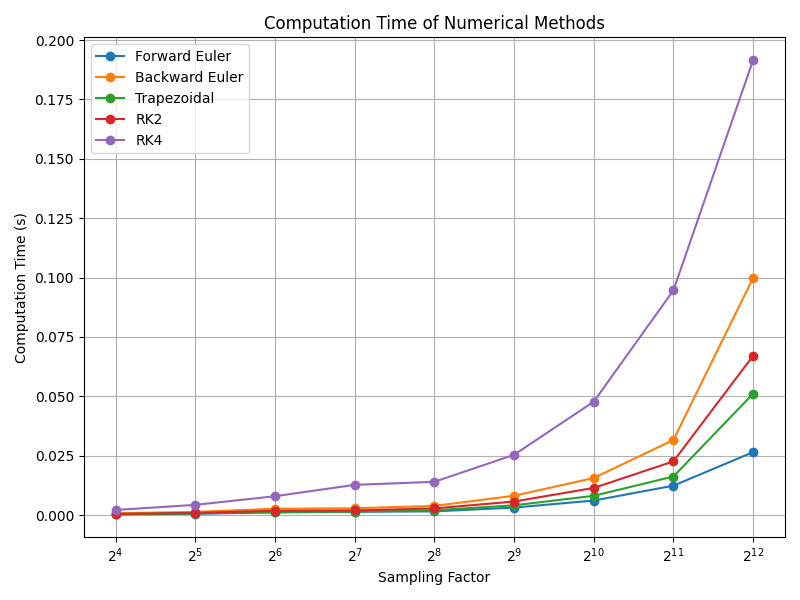
\includegraphics[width=\textwidth]{figs/computation_time.png}
  \caption{Computational times (y-axis) versus sampling factors (x-axis) for the different methods.}
  \label{fig:comp_times}
\end{figure}

